\documentclass{beamer}

\mode<presentation> 
{
    \usetheme{Madrid}
}

\usepackage[utf8x]{inputenc}
\usepackage[english,russian]{babel}
\usepackage[T2A]{fontenc}
\usepackage{graphicx}
\usepackage{booktabs} 
\usepackage{mathtools}
\usepackage{amsmath}
\usepackage{wasysym}
\usepackage{subfig}
\usepackage{hyperref}
\usepackage{ulem}
\usepackage{ragged2e}
\usepackage{algorithm2e}
\usepackage{minted}

\usemintedstyle{borland}

\usefonttheme[onlymath]{serif}

\hypersetup
{
    colorlinks=true,
    linkcolor=white, 
    urlcolor=cyan
}

\title[Лекция 0]
{
    Лекция 0: Цифровая фильтрация и \\ базовые понятия языка программирования Си
} 


\author[Д. А. Караваев]{Д. А. Караваев}

\institute[СПбГУТ] 
{
    Санкт-Петербургский государственный университет телекоммуникаций \\ им. проф. М. А. Бонч-Бруевича \\ 
    \vspace{0.2cm}
    Факультет РТС, Кафедра РОС \\
    \vspace{0.2cm}
    Факультатив <<Программирование в ЦОС>> \\
    \vspace{0.2cm}
    Осень 2019
}

\date[07.10.2019]{07.10.2019 Санкт-Петербург} 

\begin{document}
    \begin{frame}
        \titlepage 
    \end{frame}
    \begin{frame}
        \frametitle{Необходимые/приобретаемые знания}
        \begin{itemize}
            \justifying
            \item {\bf Язык программирования Си}:
            \par 
            Выразительный и, до сих пор, один из наиболее востребованных и популярных языков программирования (\url{https://www.tiobe.com/tiobe-index/}, \url{http://pypl.github.io/PYPL.html});
            \item {\bf Цифровая обработка сигналов (ЦОС)}:
            \par 
            Акцент будет сделан на задачах, возникающих в приложениях ЦОС и радиотехнике.
            \item {\bf Алгоритмы}: 
            \par 
            Будут представлены некоторые классические алгоритмы и структуры данных с примерами их приложений;
            \item {\bf Операционные системы семейства GNU/Linux}:
            \par
            Наиболее приспособлены для разработки и сопровождения ПО, часто встречаются во встроенной разработке (чем мы будем заниматься во второй части курса) и к тому же бесплатные.
        \end{itemize}
    \end{frame}
    \begin{frame}
        \frametitle{Материалы}
        \begin{itemize}
            \item Исходные файлы проектов с заданиями и материалы: \url{https://github.com/dkaravaev/bonch-dsp-faculty}.
            \item Книга: <<Язык программирования Си: лекции и упражнения>>, С. Прата;
            \item Книга: <<Теория и применения цифровой обработки сигналов>>, Л. Рабинер, Б. Гоулд;
            \item Онлайн-курс <<Программирование на языке C++>>: \url{https://stepik.org/course/7/promo};
            \item Онлайн-курс <<Digital Signal Processing>>: \url{https://www.coursera.org/learn/dsp};
            \item Дистрибутив GNU/Linux семейства Debian: Ubuntu или Linux Mint.
        \end{itemize}
    \end{frame}
    \begin{frame}
        \frametitle{КИХ-фильтр: алгоритм свёртки}
        \begin{block}{Формулировка}
            \justifying
            Реализовать цифровой фильтр с конечной импульсной характеристикой (КИХ-фильтр), который задаётся формулой свёртки:
            \begin{equation}
                y[n] = h[n] * x[n] = \sum_{k=0}^{T - 1}h[k]x[n-k], \label{eq:conv}
            \end{equation}
            где даны:
            \begin{itemize}
                \justifying
                \item входной сигнал (последовательность) $x[n]$ длины $N$: 
                      \par
                      $\{x[0], x[1], \dotsc, x[N - 1]\}$;
                \item импульсная характеристика (ИХ) $h[n]$ длины $T$,
            \end{itemize}
            и надо найти выходной сигнал $y[n]$ длины $N$.
            \end{block}
    \end{frame}
    \begin{frame}
        \frametitle{Пример}
        \begin{figure}[!tbp]
           \centering
           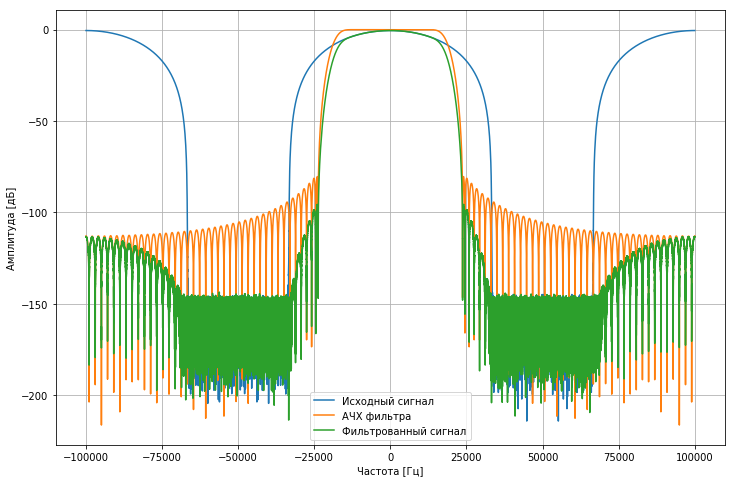
\includegraphics[width=0.85\textwidth]{pics/conv_example.png}
           \captionsetup{justification=centering}
           \captionof{figure}{Пример амплитудного спектра исходного и фильтрованного широкополосного сигнала}
       \end{figure}
    \end{frame}
    \begin{frame}
        \frametitle{Дополнение нулями}
        \justifying
        Вычисление свёртки начинается c $x[0]$ $\implies$ необходимо определить $x[n]$ для $n \in \{T - 2, \dotsc, -1\}$ (иначе сумма в $(1)$ не имеет смысла при $n \in {0, \dotsc, T - 1}$). 
        \par
        Положим: $x[n] = 0,\ n \in \{T-2, \dotsc, -1\}$.
        \par
        Операция называется {\bf дополнением нулями} ({\it англ.} zero padding), результатом которой будет последовательность длинны $N + T - 1$: 
        $$\hat x[n] = \{\hat x[0] = 0, \dotsc, \hat x[T - 1] = x[0], \dotsc, \hat x[N - T - 2] = x[N - 1]\}.$$
        Тогда формула свёртки $(1)$ будет иметь вид:
        \begin{equation}
            y[n] = h[n] * x[n] = \sum_{k=0}^{T - 1}h[k] \hat x[n + (T - 1) - k], \label{eq:conv_pad}
        \end{equation}
        которую можно разложить в два этапа $(2.1)$ и $(2.2)$ (см. далее).
    \end{frame}
    \begin{frame}{Визуализация дополнения нулями}
        \begin{figure}[!tbp]
               \centering
               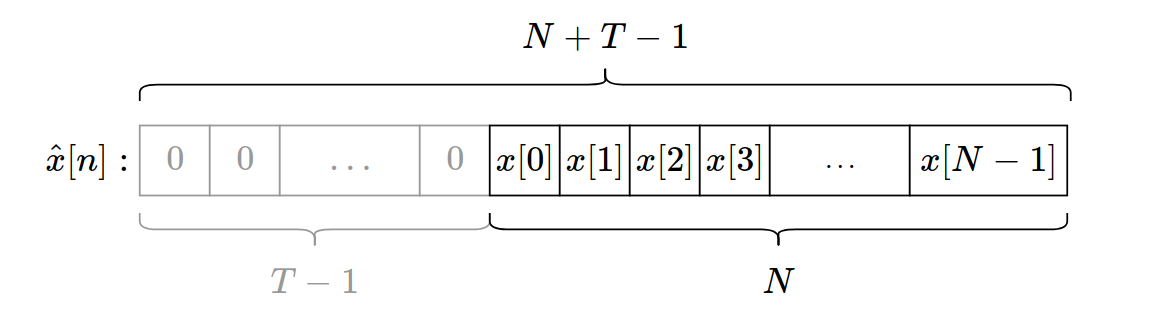
\includegraphics[width=\textwidth]{pics/padding.png}
               \captionsetup{justification=centering}
               \captionof{figure}{Результат дополнения нулями}
        \end{figure}
    \end{frame}
    \begin{frame}
        \frametitle{Визуализация алгоритма свёртки}
        \begin{figure}[!tbp]
           \centering
           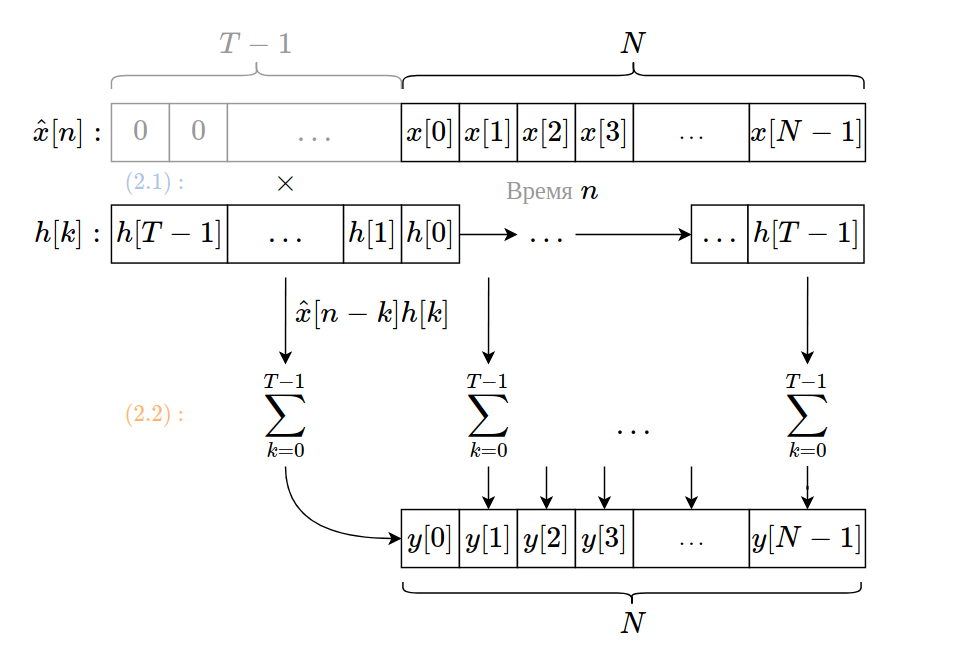
\includegraphics[width=0.85\textwidth]{pics/convolve.png}
           \captionsetup{justification=centering}
           \captionof{figure}{Схема алгоритма свёртки}
       \end{figure}
    \end{frame}
    \begin{frame}{Псевдокод алгоритма свёртки}
        \begin{algorithm}[H]
            \SetKwInOut{Input}{Вход}
            \SetKwInOut{Output}{Выход}
            \Input{$\hat x[n]$ - вх. сигнал длины $N + T - 1$, $h[n]$ - ИХ длины $T$.}
            \Output{$y[n]$ - вых. сигнал длины $N$.}
            \BlankLine
            \For(\tcp*[f]{Цикл по времени}){$n \leftarrow 0$ \KwTo $N - 1$} 
            {
                $y[n] \leftarrow 0$ \tcp*[f]{Инициализация n-ого вых. отсчёта}
                \par
                $m \leftarrow n + (T - 1)$ \tcp*[f]{Смещение по доб. нулями массиву}
                \par
                \For(\tcp*[f]{Цикл вычисления n-ого вых. отсчёта}){$k\leftarrow 0$ \KwTo $T - 1$}
                {
                    $y[n] \leftarrow y[n] + \hat x[m - k]h[k]$ \tcp*[f]{Умножение с накоплением (MAC)}
                }
            }
        \end{algorithm}
        \par
        \begin{block}{Вывод}
            Необходимо узнать как в языке Си: {\it создавать переменные и последовательности, задавать цикл со счётчиком, производить арифметические операции и операции сравнения.}
        \end{block}
    \end{frame}
    \begin{frame}[fragile]{Типы и переменные в языке Си} 
        \begin{minted}[frame=lines,        framesep=2mm,
                      baselinestretch=1.2, fontsize=\footnotesize,
                      linenos]{c}
/* Это комментарий! */
T variable; /* Объявление переменной с некоторым (псевдо)типом T. */
/* Нас интересуют числовые типы: int, float и т.д. */
float a;    /* Объявление переменной типа float. */
/* Переменным можно (и нужно) присваивать значения (=): */
a = 3.14;   /* Это называется инициализация - первичное 
             * присвоение значения. */
int x = 1;  /* Объявление с инициализацией переменной типа int. */
/* Можно (и иногда нужно) использовать модификаторы для типов: 
 * unsigned (беззнаковый) и const (неизменяемое значение). */
const unsigned int CONSTANT = 20; /* Константа типа беззнаковый int. */
        \end{minted}
        \par
        \justifying
        {\bf Вывод:} Переменная - это область памяти компьютера, к которой можно обращаться для чтения или записи по заданному имени. 
    \end{frame}
    \begin{frame}[fragile]{Арифметические операции и операции сравнения}
        \begin{minted}[frame=lines,        framesep=2mm,
                      baselinestretch=1.2, fontsize=\footnotesize,
                      linenos]{c}
/* В Си арифметические операции обозначаются стандартно: 
 * (-, +, /, *) */
float x = 1.0;
float y = 2.0;
/* Пример для +. Аналогично для: (-, *, /). */
float z = x + y; /* z: 3.0. x и y - операнды (в контексте операции). */
/* Сделать операцию с самим собой в качестве операнда: */
z += x; /* <-> z = z + x, z: 4.0. */
/* Операции сравнения: (==, !=, <, >, <=, >=). */
/* Результат: true (1) или false (0). */
int less = z < x; /* less == false. */ 
int moreq = z >= y; /* moreq = true. */
/* Приоритет исполнения операций: */
int neq = (2 * z + 1) == (2 * (z + 1)); /* neq == true. */
        \end{minted}
    \end{frame}
    \begin{frame}[fragile]{Массивы в языке Си}
        \justifying
        Для реализации алгоритма свёртки нам нужны переменные, которые бы содержали последовательность значений одного типа (например \texttt{float}). Такие переменные называются {\bf массивами}.
        \begin{minted}[frame=lines,        framesep=2mm,
                      baselinestretch=1.2, fontsize=\footnotesize,
                      linenos]{c}
/* Нумерация (индексация) массивов в Си начинается с 0, а не с 1. */
float x[10]; /* Объявление массива типа float c двумя элементами (длины 2). */
x[0] = 0.1; /* Присвоить значение 0-му элементу. */
int i = 9; /* Переменная-индекс. */
x[i] = 0.1 * i; /* Присвоить значение 9-му (последнему) элементу. */
x[i - 5] = x[i] + 3.14; /* Присвоить значение 4-му элементу. */
x[i + 4] = 0.4; /* !Ошибка!: В массиве нет 13-ого элемента. */
/* C элементами массива можно делать все тоже самое, что с 
 * обычными переменными, то есть массив это переменная, 
 * состоящая из пронумерованной последовательности 
 * других переменных (сигнал <-> массив!). */
        \end{minted}
    \end{frame}
    \begin{frame}[fragile]{Указатели в языке Си}
        \justifying
        Подобные массивы не удобны, так как они имеют заранее заданную длину. 
        В нашем случае, длины последовательностей заранее неизвестны. На помощь приходят {\bf указатели}.
        \begin{minted}[frame=lines,        framesep=2mm,
                  baselinestretch=1.2, fontsize=\footnotesize,
                  linenos]{c}
/* Указатель - это переменная, значение которой - адрес другой переменной 
 * в памяти компьютера. */
float* ptr; /* Указатель на переменную типа float. 
             * Не инциализирован (указывает в никуда). */
/* Оператор & - возвращает адрес своего аргумента (переменной). */
float y = 0.0;
ptr = &y; /* ptr указывает в адрес y (инициализирован). */ 
*ptr = 1.12; /* По указателю можно обращаться к переменной 
              * с помощью оператора (*), примененного к нему. */
/* Разименованный указатель - синоним переменной, на которую он 
 * указывает. После последней операции: y == 1.12. */
        \end{minted}
    \end{frame}
    \begin{frame}[fragile]{Указатели и массивы/Арифметика указателей}
        \begin{minted}[frame=lines,        framesep=2mm,
                  baselinestretch=1.2, fontsize=\footnotesize,
                  linenos]{c}
float x[10]; 
/* Инициализируем все значения x...*/
/* По указателю можно смещаться вправо (+) или влево (-) на n шагов. */
float* begin = &x[0]; /* Указывает на x[0] */
float* mid   = begin + 4; /* Указывает на x[4] */
int n = 3; /* Можно сделать так: */
float* second = mid - n; /* Указывает на x[1] */
/* Более того: */
begin[1] = 0.2; /* x[1] == 0.2 -> begin - это синоним имени массива! */
/* Имя массива - это указатель на его 0-вой элемент. */
        \end{minted}
        \justifying
        Таким образом последовательности неизвестной длины мы будем задавать через указатели на их 0-вой элемент и, имея переменную с длиной этой последовательность, мы не будет выходить за её пределы.
    \end{frame}
    \begin{frame}{Иллюстрация арифметики указателей}
        \begin{figure}[!tbp]
               \centering
               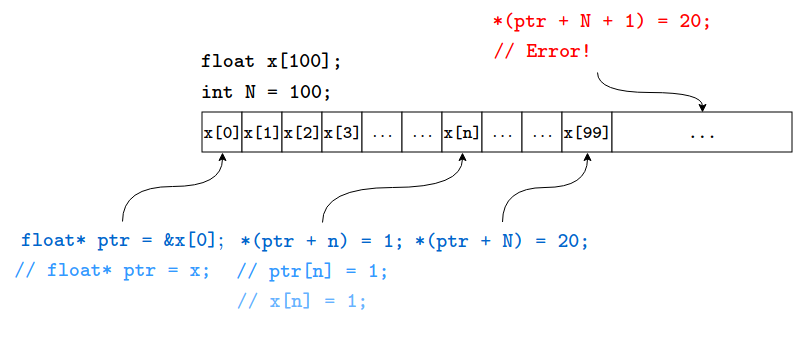
\includegraphics[width=\textwidth]{pics/ptrs.png}
               \captionsetup{justification=centering}
               \captionof{figure}{Арифметика указателей. Более тусклые цвета в комментариях - синонимичные действия.}
        \end{figure}
    \end{frame}
    \begin{frame}[fragile]{Цикл со счётчиком (\texttt{for})}
        \justifying
        Для того чтобы вычислить значения $y[n]$ нам нужно использовать цикл со счётчиком, который в языке Си определяется так:
        \begin{minted}[frame=lines,        framesep=2mm,
                       baselinestretch=1.2, fontsize=\footnotesize,
                       linenos]{c}
float array[10];
int N = 10;
for (int i = 0; i < N; i++)
{
    /* 1. int i = 0; Инициализация счётчика. */
    /* 2. i < N; Ограничение на величину счётчика. */
    /* 3. i++; Инкремент <-> i += 1 <-> i = i + 1. */
    array[i] = 0.1 * i;
}
        \end{minted}
    \end{frame}
    \begin{frame}[fragile]{Прототип функции}
        \justifying
        Алгоритм свёртки будет реализован в теле {\bf функции}. К тонкостям функций в языке Си мы ещё вернёмся. На данном этапе определим {\it прототип} функции (файл {\tt source/convolve.c}):
        \begin{minted}[frame=lines,        framesep=2mm,
                  baselinestretch=1.2, fontsize=\footnotesize,
                  linenos]{c}
int DSP_convolve(const float* xh, float* y, size_t N, 
                 const float* h, size_t T)
{
    /* N, T - длины последовательностей x[n] и ИХ фильтра соответственно,
     * xh - входная последовательность x[n] дополненная нулями,
     * y - выходная последовательность, h - ИХ фильтра. */
    /* Замечание: Тип size_t - беззнаковый целочисленный тип. */
    /* Замечание: Модификатор const у указателя говорит о том, 
     * что значение по его адресу изменить нельзя. */
    /* Далее идёт код для вычисления... ваша задача:) */
    return 0; /* Возвращающие значение функции. Об этом позже. */
}
        \end{minted}
    \end{frame}
    \begin{frame}[fragile]{Сборка}
        \justifying
        После того как код функции был написан, необходимо {\bf собрать} проект, в котором реализована 
        данная функция, то есть преобразовать код на языке Си в файл, который можно будет исполнить. Для этого в папке проекта нужно исполнить следующие команды в терминале:
        \begin{minted}[frame=lines,        framesep=2mm,
                       baselinestretch=1.2, fontsize=\footnotesize,
                       linenos]{bash}
mkdir build # Создать папку для сборки build.
cd build # Войти в папку build.
cmake .. # Настроить сборку.
make # Осуществить сборку.
        \end{minted}
        \par
        \justifying
        {\bf Замечание}: В программе могут быть {\it синтаксические} ошибки, и компилятор (программа, которая осуществляет преобразование кода на языке Си в исполняемый файл) скажет вам, где они. 
        \par
        {\bf Замечание}: Отсутствие {\it синтаксических} ошибок не означает отсутствие {\it семантических} :)!
    \end{frame}
    \begin{frame}[fragile]{Запуск и просмотр результата}
        \justifying
        После того, как проект был собран, то можно запустить полученный исполняемый файл:
        \begin{minted}[frame=lines,        framesep=2mm,
               baselinestretch=1.2, fontsize=\footnotesize,
               linenos]{bash}
# В папке build:
./convolve # Запускаем проект.
# Запускаем скрипт на языке Python для просмотра результата:
python3 ../scripts/plot_regular.py  
        \end{minted}
        {\bf Замечание}: Мы использовали системы для сборки проектов на языке Си: {\tt CMake} и {\tt Make}. О них поговорим подробнее позже.
        \par 
        {\bf Замечание}: Входной сигнал считывается из файла, а выходной записывается. На основе этих файлов, скрипт на языке {\tt Python} отображает результат работы алгоритма. 
    \end{frame}
    \begin{frame}{Визуализация результата}
        \begin{figure}[!tbp]
           \centering
           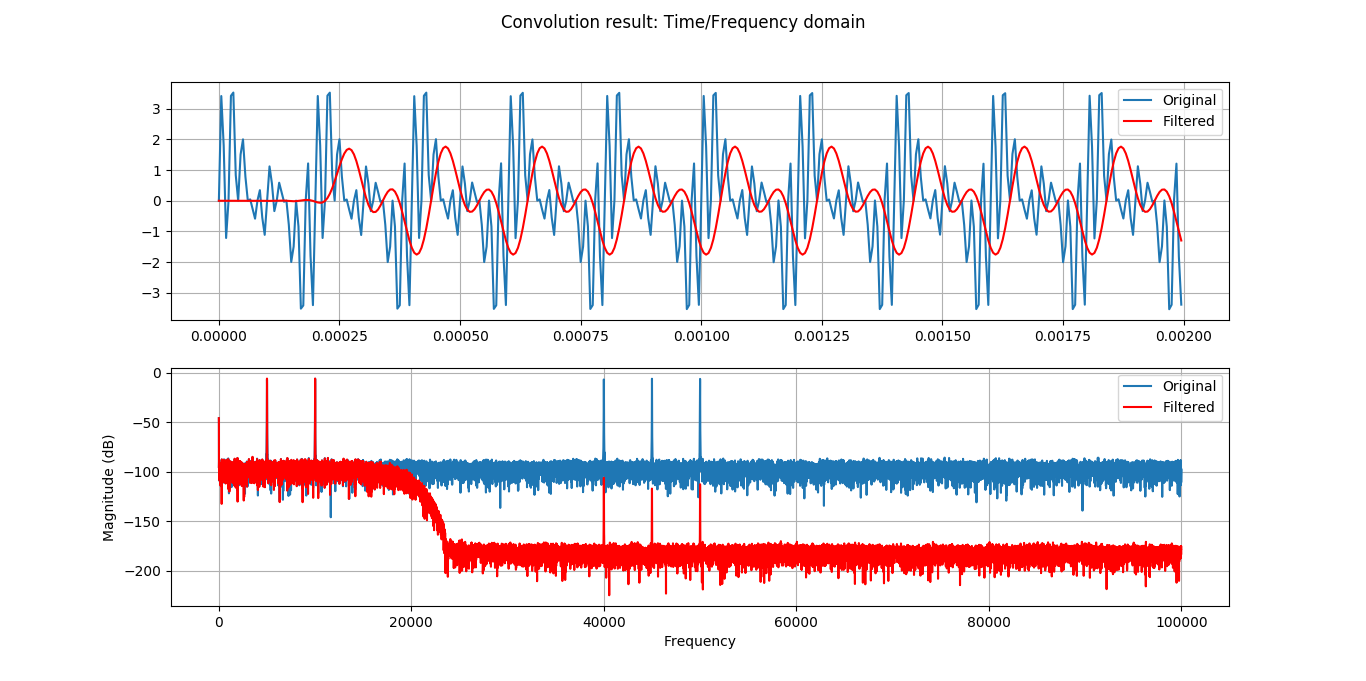
\includegraphics[width=\textwidth]{pics/result_regular.png}
           \captionsetup{justification=centering}
           \captionof{figure}{Результат фильтрации входного сигнала $x[n]$ (линейная комбинация пяти синусоид)}
        \end{figure}
    \end{frame}
    \begin{frame}{Cвёртка с децимацией$^{*}$: формулировка}
        \justifying 
        Из рисунка на предыдущем слайде видно, что подавленная фильтром часть полосы больше не представляет интереса $\implies$ можно понизить частоту дискретизации $x[n] - F_{s}$ до перехода к полосе пропускания фильтра.
        \par
        Для этого берутся только отсчёты $y[nD]$, где $D$ - коэффициент децимации, то есть формула $(2)$ будет иметь вид:
        \begin{equation}
            y[nD] = h[n] * x[nD] = \sum_{k=0}^{T - 1} h[k]\hat x[nD + (T - 1) - k] \label{eq:conv_dec}
        \end{equation}
        \par
        Частота дискретизации для $y[nD]$ равна $F_{s}/D$!
        \par
        {\bf Задача:} {\it Реализовать алгоритм свёртки с децимацией для входной последовательности $\hat x[n]$}.
        \par
        {\bf NB:} Если размер входа $x[n]$ равен $N$, то у выхода $y[nD]$ - $N/D$!
    \end{frame}
    \begin{frame}[fragile]{Cвёртка с децимацией$^{*}$: прототип функции}
        \begin{minted}[frame=lines,        framesep=2mm,
                       baselinestretch=1.2, fontsize=\footnotesize,
                       linenos]{c}
/* Прототип функции для свёртки с децимацией: */
int DSP_convolve_decimate(const float* xh, float* y, size_t N, 
                          const float* h, size_t T, size_t D)
{
    /* ... */
    /* D - коэффициент децимации. */
    return 0;
}
        \end{minted}
        \begin{figure}[!tbp]
           \centering
           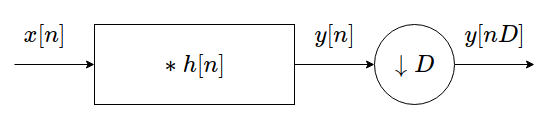
\includegraphics[width=0.8\textwidth]{pics/convdec.png}
           \captionsetup{justification=centering}
           \captionof{figure}{Схема свёртки с децимацией}
        \end{figure}
    \end{frame}
    \begin{frame}[fragile]{Cвёртка с децимацией$^{*}$: результат}
        \begin{figure}[!tbp]
           \centering
           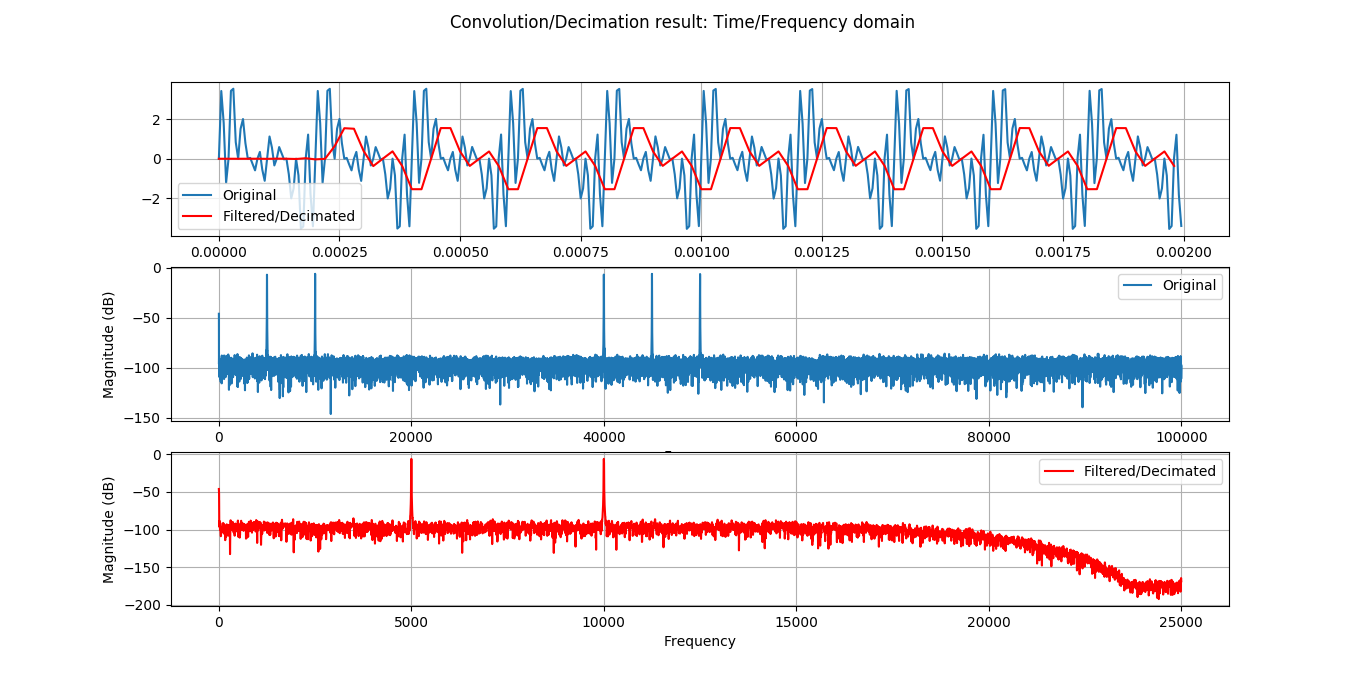
\includegraphics[width=\textwidth]{pics/result_decimated.png}
           \captionsetup{justification=centering}
           \captionof{figure}{Результат фильтрации c децимацией. Команда для отображения: {\tt python3 ../scripts/plot\_decimated.py}}
        \end{figure}
    \end{frame}
    \begin{frame}
        \begin{center}
        \baselineskip 20.0mm
        \Huge Спасибо за внимание!
        \end{center}
    \end{frame}
\end{document}